\documentclass{report}
\usepackage{fullpage}
\usepackage{stmaryrd}
\usepackage{hyperref}
\usepackage{mathtools}
% \usepackage[english]{babel}
\usepackage{enumerate}  % enumarate styles
\usepackage{url}
\usepackage[pdftex]{graphicx}
\usepackage{amsmath}
\usepackage{amsfonts}
\usepackage{galois}
\usepackage{mathabx}
\usepackage{todonotes}
\usepackage{paralist}
\usepackage{multirow}
\usepackage{caption}
\usepackage{subfigure}
\usepackage{algorithmicx}
\usepackage[noend]{algpseudocode}
\usepackage{algorithm}
\usepackage{fancyvrb}
\usepackage{lscape}
\usepackage{listings}
\usepackage{pdflscape}
\usepackage{wrapfig}
\usepackage{etoolbox}
\usepackage{tikz}
\usetikzlibrary{shapes}
\usetikzlibrary{arrows}
\usetikzlibrary{positioning}
\usetikzlibrary{automata}
\usetikzlibrary{calc}

\lstset{
  basicstyle=\ttfamily,
  mathescape
}

% \lstset{
%   language=C
% }

\sloppy
% comment the following line to bring back the margins
\IfFileExists{./tmp/rm-margin.tex}{\input{tmp/rm-margin}}{}
% \usepackage[paperheight=19.5cm,paperwidth=12.4cm,margin=.1cm]{geometry}

% \usepackage{algorithm2e}

\makeatletter
\newcommand{\dashedrightarrow}[1][2pt]{%
  \settowidth{\@tempdima}{$\rightarrow$}\rightarrow% typeset arrow
  \makebox[-\@tempdima]{\hskip-1.5ex\color{white}\rule[0.5ex]{#1}{1pt}}% typeset overlay
  \phantom{\rightarrow}% advance appropriate horizontal distance
}
\makeatother

\newcommand{\ashu}[1]{ {\textcolor{magenta} {Ashutosh: #1}} }
\newcommand{\supratik}[1]{ {\textcolor{red} {Supratik: #1}} }
\newcommand{\rahul}[1]{ {\textcolor{blue} {Divyesh: #1}} }

\newcommand{\naturals}{\mathbb{N}}
\newcommand{\integers}{\mathbb{Z}}
\newcommand{\ordinals}{\mathbb{O}}
\newcommand{\numarals}{\mathbb{I}}

\newtheorem{df}{Definition}
\newcommand{\program}{P}
\newcommand{\sassign}{\;\mathtt{:=}\;}
\newcommand{\defeq}{\triangleq}
\newcommand{\assume}{\mathtt{assume}}
\newcommand{\formulas}{\Sigma}
\newcommand{\terms}{\mathcal{T}}

\newcommand{\ltrue}{\mathbf{tt}}
\newcommand{\lfalse}{\mathbf{ff}}
\newcommand{\limplies}{\Rightarrow}
\newcommand{\lxor}{\oplus}
\newcommand{\Land}{\bigwedge}
\newcommand{\Lor}{\bigvee}
\newcommand{\Lxor}{\bigoplus}
\newcommand{\lequiv}{\Leftrightarrow}
\newcommand{\landplus}{\mathrel{:\hspace{-3pt}\land\hspace{-3pt}=}}
\newcommand{\lorplus}{\mathrel{:\hspace{-3pt}\lor\hspace{-3pt}=}}

\newcommand{\maps}{\rightarrow}

\newcommand{\union}{{\cup} }
\newcommand{\Union}{{\bigcup} }
\newcommand{\powerset}{\mathcal{P}}
\newcommand{\intersection}{{\cap} }
\newcommand{\Intersection}{{\bigcap} }
\newcommand{\compose}{{\circ} }

\newcommand{\locationOf}[1]{loc(#1)}

\newcommand{\formula}{\phi}
\newcommand{\preds}{\pi}
\newcommand{\domain}{\mathcal{D}}

\newcommand{\smem}{\mathcal{S}}
\newcommand{\tout}{TO}


%algorithm names
\newcommand{\concolic}{concolic}

\newcommand{\correct}{\textsc{CORRECT}}

\newcommand{\qfbv}{\texttt{QF\_BV}}

%tool names
% \newcommand{\ourtool}{$\crest^{+}$}
\newcommand{\ourtool}{\textsc{Crabs}}
\newcommand{\zthree}{\textsc{Z3}}
\newcommand{\cvcfour}{\textsc{CVC4}}
\newcommand{\crest}{\textsc{Crest}}
\newcommand{\synergy}{\textsc{Synergy}}
\newcommand{\cpachecker}{\textsc{CpaChecker}}
\newcommand{\fshell}{\textsc{Fshell}}
\newcommand{\svcomp}{\textsc{SvComp}}
\newcommand{\tiger}{\textsc{CpaTiger}}
\newcommand{\tara}{\textsc{Tara}}
\newcommand{\doublemp}{\mathtt{double\text{-}mp}}

\newcommand{\musketeer}{\textsc{Musketeer}}
\newcommand{\fender}{\textsc{Fender}}
\newcommand{\blender}{\textsc{Blender}}
\newcommand{\dfence}{\textsc{Dfence}}
\newcommand{\remmex}{\textsc{Remmex}}
\newcommand{\memorax}{\textsc{Memorax}}
\newcommand{\pensieve}{\textsc{Pensieve}}
\newcommand{\trencher}{\textsc{Trencher}}
\newcommand{\persist}{\textsc{Persist}}
\newcommand{\glue}{\textsc{Glue}}

\newcommand{\intel}{\textsc{Intel}}
\newcommand{\arm}{\textsc{ARM}}
\newcommand{\sparc}{\textsc{Sparc}}

\newtheorem{thm}{Theorem}

\newcommand{\rndbr}{RndBr}
\newcommand{\unfrnd}{UnfRnd}

%--------------------- DO NOT ERASE BELOW THIS LINE --------------------------

%%% Local Variables: 
%%% mode: latex
%%% TeX-master: "main"
%%% End: 


\setcounter{tocdepth}{10}
\setcounter{secnumdepth}{10}

\pagestyle{plain}

\begin{document}

\title{Matching Multiplications in Bit-Vector formulas\footnote{to appear in Proc. of International Conference on Verification, Model Checking and Abstract Interpretation (VMCAI), January 2017}}


%Names are in alphabetical order
%\author{Rahul Jain}
%\institute{School of Technology and Computer Science, Tata Institute of Fundamental Research}
%Supratik Chakraborty$^1$ \and Ashutosh Gupta$^2$ acknowledge 

%\date{\today}

\author{Rahul Jain}
\affil{School of Technology and Computer Science \\Tata Institute of Fundamental Research \\Mumbai}

\date{Dated: \today}

\maketitle

\begin{abstract}
%
On an input bit-vector formula,
a typical SMT solver proceeds by applying several
simplification rules and then bit-blasting.
%
The bit-vector formulas with multiplications
are particularly hard for SMT solvers.
%
Therefore, it becomes more important that the simplification detects
high level structures in the formulas in order to solve it faster.
%
In this paper, we present a class of simplifications that may be
needed in solving formulas containing multiplications and no leading
solver implements it, and an efficient algorithm to recognize the
simplification pattern. 
%
We have added the algorithm in rewriting engine of $\zthree$
and applied on benchmarks.
%
Our modification solves several formulas that are
intractable by any other leading solver.
%

%--------------------- DO NOT ERASE BELOW THIS LINE --------------------------

%%% Local Variables: 
%%% mode: latex
%%% TeX-master: "main"
%%% End: 

\end{abstract}


\centerline{\bfseries Acknowledgements}
\vspace{0.2 cm}

I would like to thank

\clearpage
\tableofcontents

%
\chapter{Introduction}
\label{sec:intro}
% Bit-vector is important
%
In recent years, SMT solving has emerged as a powerful technique for
testing, analysis and verification of hardware and software systems.
A wide variety of tools today use SMT solvers as part of their core
reasoning engines; examples include bounded model
checkers~\cite{hwcbmc,boolector,ebmc,cbmc}, static assertion
checkers~\cite{corral,boogie}, word-level symbolic trajectory
evaluators~\cite{wste}, constrained test
generators~\cite{crv1,crv2,dart}, concolic simulators~\cite{concolic},
among others.  A common approach used by these tools is to model the
behaviour of a system using formulas in a combination of first-order
theories, and reduce the given problem to checking the
(un)satisfiability of a formula in the combined theory.  SMT solvers
play a central role in this scheme of things, since they combine
decision procedures of individual first-order theories to check the
satisfiability of a formula in the combined theory.  Not surprisingly,
techniques to improve the performance of SMT solvers have attracted
significant attention over the years.  The literature contains a rich
body of heuristic strategies for improving the performance of
theory-specific solvers (see~\cite{barrett,deMoura2013} for excellent
expositions).  In this paper, we add to the repertoire of such
heuristics by proposing a pre-processing step that conjoins an input
formula with specially constructed assertions, without changing its
semantics. We focus on formulas in the quantifier-free theory of
fixed-width bit-vectors with multiplication, and show by means of
experiments that our pre-processing heuristic yields significant
performance benefits in many cases for three state-of-the-art SMT
solvers, namely {\zthree}~\cite{zthree}, {\cvcfour}~\cite{cvcfour} and
{\boolector}~\cite{boolector}.  Significantly, our heuristic helps
reduce the solving time for multiple examples by upto several orders
of magnitude when the input formula is unsatisfiable.

%% Theories commonly
%% supported in modern SMT solvers include the quantifier-free theories
%% of fixed-width bit-vectors, arrays, lists, strings, among
%% others~\cite{kroening-book,smtlibv2}.
%% Since reasoning in these individual theories is often much more
%% efficient than reasoning about the bit-level representation of the
%% corresponding data types, techniques based on SMT solving hold a lot
%% of promise as far as scaling to large applications is concerned.  The
%% impressive progress made in SMT solving over the last two
%% decades~\cite{smtprogress} has also substantially lived up to this
%% hope. 

The primary motivation for our work comes from word-level bounded
model checking (WBMC)~\cite{cbmc,hwcbmc} and word-level symbolic
trajectory evaluation (WSTE)~\cite{wste} of embedded hardware systems.
Specifically, we focus on systems that process data, represented as
fixed-width bit-vectors, using arithmetic operators.  Examples of such
systems include digital signal processing filters, graphics
accelerators, encryption and decryption modules, custom datapath
implementations etc.  When reasoning about these systems, it is often
necessary to check whether a high-level property, specified using
bit-vector arithmetic operators (viz. addition, multiplication,
division), is satisfied by a model of the system implementing a
data-processing algorithm.  For reasons related to performance, power,
area, ease of design etc., complex arithmetic operators with large
bit-widths are often implemented by composing several smaller, simpler
and well-characterized blocks.  For example, a $128$-bit multiplier
may be implemented using one of several multiplication algorithms,
viz. long multiplication~\cite{long}, Booth-encoded
multiplication~\cite{booth} or Wallace-tree
multiplication~\cite{wallace}, after partitioning its $128$-bit
operands into narrower, say $8$-bit wide, blocks.  SMT formulas
resulting from WBMC/WSTE of such systems are therefore likely to
contain terms with higher-level arithmetic operators (viz. $128$-bit
multiplication) encoding the specification, and terms that encode a
lower-level implementation of these operators in the system (viz. a
Wallace-tree multiplier).  Efficiently reasoning about such formulas
requires exploiting the semantic equivalence of these alternative
representations of arithmetic operators.  Unfortunately, our study,
which focuses on systems using the multiplication operator, reveals
that three state-of-the-art SMT solvers ({\zthree}, {\cvcfour} and
{\boolector}) encounter serious performance bottlenecks in identifying
these equivalences.  This manifests dramatically when reasoning about
the unsatisfiability of formulas.

\noindent {\bfseries \emph{A motivating example:}} To illustrate
the severity of the problem, we consider the SMT formula arising out
of WSTE applied to a pipelined serial multiplier circuit, originally
used as a benchmark in~\cite{wste}.  The circuit reads in two $32$-bit
operands sequentially from a single $32$-bit input port and stores
them in internal registers, before multiplying them and making the
$64$-bit result available in an output register.  The circuit also has
several control signals that can be used to change the flow of
control, effectively delaying the computation of the result.

The property to be checked asserts that if $a$ and $b$ denote the two
operands that are read in, then after the computation is over, the
output register indeed has the product $a *_{[32]} b$, where
$*_{[32]}$ denotes $32$-bit multiplication.  The RTL design
(i.e. system implementation), as used in~\cite{wste}, makes use of the
{\tt *} operator in $\sysver$, with $32$-bit operands.  The Language
Reference Manual of $\sysver$ specifies that this amounts to using a
$32$-bit multiplication operation directly.  The SMT formula resulting
from a WSTE run on this example therefore contains terms with only
$32$-bit multiplication operators, and no terms encoding a lower-level
multiplier implementation.  This formula is shown to be unsatisfiable
within a fraction of a second by {\boolector} (and also by {\cvcfour}
and {\zthree}).  Note that in WSTE (as also in WBMC), the SMT formula
encodes violation of a property by a bounded run of the system. Hence,
unsatisfiability of the formula implies the absence of any bounded
violating runs.

We now change the RTL in the above example to reflect the
implementation of $32$-bit multiplication by the long-multiplication
algorithm~\cite{long}, where each $32$-bit operand is partitioned into
$8$-bit blocks.  The corresponding WSTE run yields an SMT formula that
contains terms with $32$-bit multiplication operator (derived from the
property being checked), and also terms that encode the implementation
of a $32$-bit multiplier using long-multiplication.  Surprisingly, none
of {\boolector}, {\cvcfour} and {\zthree} succeeded in deciding the
satisfiability of the resulting formula even after $24$ hours on the
same computing platform.  The heuristic strategies in these solvers
failed to identify the semantic equivalence of terms encoding
alternative representations of $32$-bit multiplication, and proceeded
to bit-blast the formulas, leading to this dramatic run-time blowup.

\noindent {\bfseries \emph{Problem formulation:}} 
The above example demonstrates that the inability to identify semantic
equivalence of alternative representations of arithmetic operators
plagues multiple state-of-the-art SMT solvers.  Therefore, a heuristic
that helps in this respect and is generic (not solver-specific) would
be highly desirable.  This motivates us to ask: \emph{Can we
pre-process an SMT formula containing terms encoding alternative
representations of bit-vector arithmetic operators, in a
solver-independent manner, so that multiple solvers benefit from it?}
We answer this question positively in this paper for the
multiplication operator.  Note, however, that like all heuristics, we
cannot guarantee that our pre-processing step helps in every case.
The motivating example, that originally timed out after $24$ hours on
three solvers, is shown to be unsatisfiable by {\zthree} in 0.073s and
by {\cvcfour} in 0.017s, after application of our heuristic. However,
{\boolector} does not benefit from our heuristic in this example.
Nevertheless, there are several other examples where {\boolector}
benefits significantly, as discussed in Section~\ref{sec:experiments}.

\noindent {\bfseries \emph{Term re-writing vs adding tautological assertions:}} 
Prima facie, the above problem can be solved by reverse-engineering
the lower-level implementation of a bit-vector arithmetic operator,
and by re-writing terms encoding the lower-level implementation with
terms using the bit-vector operator.  Indeed, variants of this
approach have been used by earlier researchers in different
contexts~\cite{kunz,ciesielski,kolbl,reveng,earlier-pat-match-synopsys}.
In the context of SMT solving, however, complications can potentially
arise if we simply re-write a term encoding one representation of an
arithmetic operator by another term encoding a different
representation of the same operator. For example, as shown in Example
$2$ of Section~\ref{sec:long-mult}, the same collection of
sums-of-partial-products arising from long-multiplication can be
obtained from two different bit-vector multiplication operations.
This makes it difficult to determine which term re-writes should be
used to help the SMT solver decide the satisfiability of the input
formula.  Furthermore, even if we are able to uniquely identify the
equivalence of two terms representing the same arithmetic operation,
re-writing one term with another may not correlate with improved solver
performance for various reasons.  Indeed, re-writing one term by
another is a ``peep-hole'' transformation that is oblivious of the
overall context in which the terms appear in the SMT formula.  What
appears beneficial locally may not be beneficial in the overall
(un)satisfiability check.  In addition, syntactially distinct terms
that are semantically equivalent may play different roles when
reasoning about different sub-formulas of an SMT formula.  For
example, one term may enable a re-write rule that helps simplify one
sub-formula, while a syntactically distinct but semantically
equivalent term may enable another re-write rule that helps simplify
another sub-formula. Re-writing one term by another precludes the
possibility of both terms contributing to improving the performance of
the overall satisfiability check.

Thus, re-writing a term encoding a specific implementation of a
bit-vector arithmetic operator with another term encoding another
implementation of the operator may not help in all cases.  In this
paper, we present a heuristic alternative to address the above
problem, focusing only on bit-vector multiplication.  Given a
bit-vector formula $\varphi$ that contains terms with two different
representations of bit-vector multiplication, our heuristic searches
for patterns corresponding to two multiplication algorithms (long
multiplication and Wallace-tree multiplication) in the terms. Instead
of re-writing the matched sub-terms directly, as has been done in
earlier work, we conjoin the formula $\varphi$ with additional
assertions that equate a matched sub-term with the corresponding
bit-vector arithmetic operator.  Note that each added assertion is a
tautology, and hence does not change the semantics of the formula.
Significantly, since no re-writes are done, we can express multiple
semantic equivalences without removing any syntactic term from the
formula.  This is an important departure from earlier techniques, such
as~\cite{kolbl}, that rely on sophisticated re-writes of the
formula. Our experiments show that the added tautological assertions
succeed in preventing bit-blasting in several cases, while in other
cases they help in pruning the search space even after bit-blasting.
Both effects eventually translate to improved performance of the SMT
solver.  Since our heuristic simply pre-processes the input formula by
adding assertions, it is independent of the internals of any specific
solver, and can be used with multiple solvers.  Our experiments show
that the performance of different SMT solvers on the pre-processed
formulas can vary.  Hence, we propose a portfolio approach to solving
the pre-processed formulas.  We show experimentally that a portfolio
solver using pre-processed formulas significantly outperforms a
portfolio solver using the original formulas.



%% Many hardware and software verification problems are translated to the
%% satisfiability of quantifier free bit-vector(QF\_BV)
%% formulas~\cite{hardware,cbmc,more}.
%


\chapter{Preliminaries}
\label{sec:prelim}
In this section, we will present syntax of
the theory of quantifier-free bit vector formulas(\qfbv),
basics of solving methods used by SMT solvers,
and the multiplication methods that are of our interest. 

\subsection{\qfbv~syntax}

A bit-vector is a fixed sequence of bits.
%
We will denote bit vectors by $x$,$y$,$z$...

Syntax of bit-vector formulas

A bit-vector $v$

\subsection{SMT solvers for \qfbv}

The leading SMT solvers for \qfbv~apply several simplification
passes followed by bit-blast, i.e. translating input to Boolean
satisfiability problem.
%
The bit-blasted SAT problem is solved using conflict driven clause
learning(CDCL) based procedures.
%




\subsection{Multipliers}



\subsubsection{Grade school multiplication}

Describe it in our $\qfbv$

\ashu{2-3 line why this definition and what to expect in the words already 
introduced}

\rahul{ We need to do this}

\begin{df}
  
\end{df}

Some discussion about the definition.

\begin{example}
  
\end{example}


\subsubsection{Wallace tree multiplier}

\subsubsection{Booth multiplier}


%\subsection{Verification problem to SMT formula}



%--------------------- DO NOT ERASE BELOW THIS LINE --------------------------

%%% Local Variables: 
%%% mode: latex
%%% TeX-master: "main"
%%% End: 


\chapter{Pattern detection}
\label{sec:pattern}
In this section, we will present a class of simplification patterns that
may simplify the formulas with multipliers 
and the algorithms to detect the patterns.


\subsection{Identifying grade school multiplication}

\subsection{Identifying Wallace tree}

\subsection{Partial products to operands}

\begin{algorithm}[t]
 \caption{\textsc{getMultOperand}($\Lambda$)}
 \label{alg:hb}
 \begin{algorithmic}[1]
   \Ensure $\Lambda$ : array of multisets of the partial products
   \State $m$ : candidate multiplier 
   \State $n$ : candidate multiplicand
   \State Choose largest $k$ such that $\Lambda_k\neq \emptyset$
   \If{$\Lambda_k == \{a*b\} $}
   \State $m_k := a; n_k := b$; $backtrack_k := \lfalse$; 
   \Else
   \State \Return{ FAILED}
   \EndIf
   \State $i := k$
   \While{ $i > 0$}
   \State $i = i - 1 $
   \State $C := \Lambda_i$
   \For{ $j \in (k-1)..(i+1)$}
   \If{$m_{j} \neq 0$ and $n_{k+i-j} \neq 0$}
   \IIf{ $m_j*m_{k+i-j} \not\in C$} {\bf goto }{\textsc{Backtrack}}
   \State $C := C - \{m_j*m_{k+i-j}\}$
   \EndIf
   \EndFor
   % \IIf{ $|C| > 2$} {\bf goto }{\textsc{Backtrack}}
   \State {\bf match} $C$ {\bf with}
   \State\quad $\mid$ $\{m_k*b,n_k*d\}$ $\rightarrow$ $m_i := d; n_i := b$;
   $backtrack_i := (m_k == n_k)$; 
   \State\quad $\mid$ $\{m_k*n_k\}$ $\rightarrow$ $m_i := 0; n_i := m_k;$
   $backtrack_i := \ltrue$; 
   \State \quad$\mid$ $\{m_k*b\}$ $\rightarrow$ $m_i := 0; n_i := b;$
   $backtrack_i := (m_k == n_k)$; 
   \State \quad $\mid$ $\{n_k*b\}$ $\rightarrow$ $m_i := b; n_i := 0;$\
   $backtrack_i := \lfalse$; 
   \State \quad $\mid$ $\{\}$ $\rightarrow$ $m_i := 0; n_i := 0;$\
   $backtrack_i := \lfalse$; 
   \State \quad $\mid$ $\_$ $\rightarrow$ {\bf goto }{\textsc{Backtrack}};
   \State {\bf continue;}
   \State \textsc{Backtrack:}
   \State \quad Choose smallest $i' \in k..(i+1)$ such that $backtrack_{i'} == \ltrue$
   \State \quad {\bf if} no $i'$ found {\bf then} \Return{ FAILED}
   \State \quad $i := i'$
   \State \quad \textsc{SWAP}($m_i,n_i$); $backtrack_{i} := \lfalse$
   \EndWhile
   \State Let $l$ be the smallest number such that $\Lambda_l\neq \emptyset$
   \State Choose $o \in 0..l$\ashu{More constraints over $o$ needed?!!}
   \State Right shift $m$ until $o$ trailing $0$ blocks in $m$
   \State Right shift $n$ until $l-o$ trailing $0$ blocks in $n$
   \State \Return $(m,n)$
 \end{algorithmic}
\end{algorithm}  

%--------------------- DO NOT ERASE BELOW THIS LINE --------------------------

%%% Local Variables:
%%% mode: latex
%%% TeX-master: "main"
%%% End:


%--------------------- DO NOT ERASE BELOW THIS LINE --------------------------

%%% Local Variables:
%%% mode: latex
%%% TeX-master: "main"
%%% End:


\chapter{Correctness}
\label{sec:correct}
We need to prove that each $[x*y = t]$ added in $\textsc{OurSolver}$
is a valid formula.
%
First we will prove the correctness of $\textsc{getMultOperands}$.
%
If either of $x$ or $y$ is zero, we assume term $x*y$ is also simplified to zero.
\begin{thm}
 If $ x*y \in \textsc{getMultOperands}(\Lambda,w)$, then
 $$
 \Lambda_i = \{ x_1*y_{i-1},....,x_{i-1}*y_1 \}
 $$
  where $x_k$ and $y_k$ are the $k$th block of $x$ and $y$ of size
$w$, respectively.
\end{thm}
\begin{proof}
  After each iteration of the loop at line 8,
  the loop body ensures that the following holds, which readers 
  may easily check.
  Otherwise, it jumps to backtracking.
  $$
  \Lambda_i = \{ x_h*y_{i}, x_{h-1}*y_{i+1},....,x_{i}*y_h \}
  $$
  Due to the above equation,
  if $x_j*y_k \in \Lambda_i$, then $ i = h-j-k$.
  %
  If the program enters at line 25, it has a successful match and $i=1$.
  Since $h-l_x -l_y \geq 1$, $\Lambda_l = \{x_{l_x}*y_{l_x}\}$
  and $l = h - l_x - l_y$.
  %
  We choose $o \leq l$, and shift $x$ and $y$ according to lines 26-27.
  After the shift, we need to write the above equation as follows.
  $$
  \Lambda_i = \{ x_{h-(l_x-o)}*y_{i-(l_y-l+o)},...,x_{i-(l_x-o)}*y_{h-(l_y-l+o)} \}.
  $$
  We can easily verify that the sum of the indexes in each of
  the partial products is $i$.
  %
  Since all $x_k$ is zero for $k > h-(l_x-o)$ and all $y_k$ is zero
  for $k > h-(l_y-l+o)$,
  we may rewrite the above equation as follows.
  $$
  \Lambda_i = \{ x_1*y_{i-1},....,x_{i-1}*y_1 \}.
  $$
\end{proof}

\begin{thm}
  If $m*n\in$ \textsc{MatchLong}$(t)$, $[m*n = t]$ is valid.
\end{thm}
\begin{proof}
  We collect partial products with appropriate offsets $o$ at line 5.
  %
  The pattern of $t$ indicates that the net result is the sum of the 
  partial products at the respective offsets. 
  %
  $\textsc{getMultOperands}(\Lambda,w)$ returns exactly the
  matches that produces the sums.
  %
  Therefore, $[m*n = t]$ is valid.
\end{proof}

\begin{thm}
  If $m*n\in$ \textsc{MatchWallaceTree}$(t)$, $[m*n = t]$ is valid.
\end{thm}
\begin{proof}
  \ashu{poorly written needs rewrite.}
  All we need to show that $t$ is intending to sum the partial products
  stored in $\Lambda$. Rest of the proof follows the previous theorem.
  
  Each bit $t_i$ must be the sum of the partial products $\Lambda_i$ and 
  the carry bits produced by the sum for $t_{i-1}$.
  %
  The algorithm identifies the terms that are added to obtain $t_i$.
  %
  Only need to prove that the terms that are not identified as
  partial products are carry bits of the sum for $t_{i-1}$.
  %
  Let us consider such a term $t$.
  %
  Let us suppose the algorithm identifies $t$ as an output of the carry
  bit circuit of a full adder (half adder case is similar) with inputs
  $a$, $b$, and $c$.
  %
  If $a$, $b$, $a \lxor b$ and $c$ are the intermediate
  results of the sum for $t_{i-1}$.
  %
  Therefore, $t$ is one of the carry bit.
  %
  Since $a$, $b$, $a \lxor b$ and $c$ are removed from $\Delta_{i-1}$
  after the match of the adder,
  all the identified adders are disjoint.
  %
  Since we require that all the elements of $\Delta_{i-1}$  are eventually
  removed except $t_{i-1}$, all carry bits are added to obtain $t_i$.
  %
  Therefore, $\Lambda$s carry the expected partial products of a Wallace tree.
\end{proof}

%--------------------- DO NOT ERASE BELOW THIS LINE --------------------------

%%% Local Variables:
%%% mode: latex
%%% TeX-master: "main"
%%% End:


\chapter{Experiments}
\label{sec:experiments}


We have implemented our algorithms as a part of $\zthree$~\cite{z3} SMT solver.
%
 We evaluate the performance of our algorithms using benchmarks that are industrial and handcrafted hardware verification problems.
%
We compare with $\zthree$, $\boolector$\cite{boolector} and $\cvcfour$\cite{cvc4}.
%
Our experiments show that the solvers time out on the benchmarks and our implementation produces results within the time limit.

Our implementation of the algorithms in $\zthree$ is 1500 lines long.
%
The algorithms have been implemented in the bit vectors rewrite module of $\zthree$.
%
We chose to work in the rewrite module, since it gives an easy access to the abstract syntax tree of the input formula.
%
One important aspect in the implementation is the ability to exit as early as possible if the match is going to fail.
%
We implemented various preliminary checks \rahul{add some checks}.
%
Our implementation has two modes.
%
In the first mode we insert the learnt tautologies in the $\zthree$ solver within the current execution.
%
In the second mode other we do not run  the $\zthree$ solver and print the learnt tautologies in a file along with the input formula.
%
The mode allows us to run the other solvers on the newly generated formula.

Our experiments include x benchmarks.
%
We received an industrial hardware verification benchmark in $\sysver$ involving long multiplication that was not solved by any of the solvers in 24 hours.
%
The example inspired our current work and to evaluate it we generated several similar benchmarks.
%
For long multiplication, we generated benchmarks by varying three characteristics, namely total bit length of the input bit-vectors, width of each block, and assigning specific blocks as equal or set them to zero.
%
Our $\sysver$ benchmarks are fed to STEWord~\cite{Word-level-Symbolic-Trajectory-Evaluation}, a hardware verification tool.
%
STEWord takes $\sysver$ design as input and generates the corresponding SMT1 formula.
%
We convert the SMT1 formula to SMT2 format using $\boolector$.
%
In the process, $\boolector$ extensively simplifies the input formula but retains the overall structure.
%
We have generated benchmarks also for Wallace tree multiplier similar to the long multiplication.
%
For $n$-bit Wallace tree multiplier, we have written a script that takes $n$ as input and generates all the files needed as input by STEWord.
%


We run the solvers on the SMT2 formulas corresponding to the benchmarks by running the solvers on the original input formula and the modified formula after adding the new tautologies.
%
For $\zthree$ we also capture the time taken to solve when the tautologies are added during the current execution.

Shorthand, $O$ - original input formula, $M$ - Generated formula, $T$ - trunk version of solver, $CE$ - $\zthree$ - Continue execution after adding tautologies, $bool$ - Boolector.
The tables below specify the results obtained on the various benchmarks.
%

\begin{table}[]
\centering
\caption{Long multiplication}
\label{my-label}
\begin{tabular}{|c|c|c|c|c|c|c|c|}
\hline
                      & \multicolumn{3}{c|}{SMT Solver} & \multicolumn{3}{c|}{Our Solver} &          \\ \hline
Benchmark             & Z3        & Boolector  & CVC4   & Z3        & Boolector  & CVC4   & Z3       \\ \hline
base                  & 2m48.51s  & 44.50s     & 18.37s & 0.48s     & 46.0s      & 0.02s  & 0.39s    \\ \hline
ex1\_scaledup         & t/o       & t/o        & t/o    & 1.65s     & t/o        & 0.02s  & 1.50s    \\ \hline
ex2\_scaledup         & t/o       & t/o        & t/o    & 3.05s     & t/o        & 0.02s  & 2.57s    \\ \hline
ex3\_scaledup         & t/o       & t/o        & t/o    & 2.84s     & 7m52.39s   & 0.03s  & 2.78s    \\ \hline
ex5\_scaledup\_2      & 5m29.56s  & 52.06s     & 39.89s & 4m51.89s  & 16.46s     & 0.02s  & 4m32.39s \\ \hline
mult\_3operands       & t/o       & t/o        & t/o    & t/o       & t/o        & t/o    & t/o      \\ \hline
sv\_assy              & t/o       & t/o        & t/o    & 0.02s     & t/o        & 0.02s  & 0.06s    \\ \hline
mot\_base\_scaledup   & t/o       & t/o        & t/o    & 14.20s    & t/o        & 0.02s  & 11.81s   \\ \hline
mot\_ex1\_scaledup\_2 & t/o       & t/o        & t/o    & t/o       & 18.43s     & 0.02s  & t/o      \\ \hline
mot\_ex2\_scaledup\_2 & t/o       & t/o        & t/o    & t/o       & 15.57s     & 0.02s  & t/o      \\ \hline
\end{tabular}
\end{table}




Explanation: 

\begin{table}[]
\centering
\caption{Wallace tree multiplier}
\label{my-label}
\begin{tabular}{|c|c|c|c|c|c|c|c|}
\hline
                & \multicolumn{3}{c|}{SMT Solver} & \multicolumn{3}{c|}{Our Solver} &       \\ \hline
Benchmark       & Z3       & Boolector & CVC4     & Z3      & Boolector   & CVC4    & Z3    \\ \hline
wallace\_4bits  & 0.08s    & 0.04s     & 0.04s    & 0.02s   & 0.05s       & 0.05s   & 0.08s \\ \hline
wallace\_8bits  & 3m33.33s & 1m3.80s   & 3m32.79s & 0.05s   & 30.60s      & t/o     & 0.44s \\ \hline
wallace\_12bits & t/o      & t/o       & t/o      & 0.09s   & 3m47.17s    & t/o     & 1.20s \\ \hline
wallace\_16bits & t/o      & t/o       & t/o      & 0.16s   & 11m28.19s   & t/o     & 2.26s \\ \hline
\end{tabular}
\end{table}


Explanation:



%--------------------- DO NOT ERASE BELOW THIS LINE --------------------------

%%% Local Variables: 
%%% mode: latex
%%% TeX-master: "main"
%%% End:



 




 \chapter{Related Work}
 \label{sec:related}
 
%--------------------- DO NOT ERASE BELOW THIS LINE --------------------------

%%% Local Variables: 
%%% mode: latex
%%% TeX-master: "main"
%%% End: 

The quest for heuristic strategies for improving the performance of
SMT solvers dates back to the early days of SMT solving.  The list of
papers that describe heuristics for SMT solving is a long and
illustrious one.  Instead of citing these individual papers, we point
the reader to an excellent exposition on this topic
in~\cite{deMoura2013}, which also makes a strong case for developing
languages that enables users to choose their preferred heuristics and
tactics in SMT solvers.

The works that come closest to our work are those developed in the
context of verifying hardware implementations of word-level
arithmetic.  Heuristics for identifying bit-vector (or word-level)
operators from gate-level implementations of these operators have been
developed and optimized by the hardware verification community for
long~\cite{kunz,ciesielski,reveng,earlier-pat-match-synopsys}.  The
use of canonical representations of bit-vector arithmetic operations
have also been explored, as in~\cite{bmd,drechsler}, among others.
These efforts were primarily intended to simplify word-level reasoning
about circuits, and to verify that implementations of complex
arithmetic operators like multiplication indeed implement the
semantics of multiplication.  None of these works were, however,
really targeted at developing SMT solving heuristics for the theory of
fixed-width bit-vectors.

The use of alternative representations of arithmetic operators has
typically been used in SMT solvers when bit-blasting high-level
operators.  For example, {\zthree}~\cite{zthree} uses a specific
Wallace-tree implemention of multiplication when bit-blasting
multiplication operations.  Similar heuristics are also followed in
other solvers like {\boolector}~\cite{boolector} and
{\cvcfour}~\cite{cvcfour}.  However, none of these are intended to
help improve the performance (run-time) of the solver when reasoning
about bit-vector formulas. 


\chapter{Conclusion and future work}
\label{sec:conclusion}
We have shown how adding tautological assertions that assert the
equivalence of different representations of bit-vector multiplication
can siginificantly improve the performance of SMT solvers.  We are
currently extending our procedure to support Booth multiplier and
other more complex arithmetic patterns.  We are also working to add
proof generation support for the added tautological assertions.  We
could not include proof generation in this work, since the basic
infrastructure of proof generation is missing in $\zthree$~bit-vector
rewriter module.
%
%We are also planning to request \zthree~team to adopt our modification in their
%standard distribution.

We plan to extend our work to problems involving different
combinations of multiplications. For example, $(X*(Y*Z))*W$ involves
three multiplications. We could chose to specify the implementation of
the three multiplications to be either of Long, Wallace, Booth
multiplication or an unspecified multiplication. To enable the pattern
detection in arbitrary arithmetic formulas, we are working to modify
the word level reasoning in the solvers.
We could further extend our work to complicated word level formulas involving bit vector multiplication like $X*X + Y*Y$, $X*(Y+Z)$, $(X*(Y*Z))*W$.

None of the solvers were able to make use of the added tautologies(one for each long multiplication). 
The problem seems to be on two fronts: one is that to check equality of two terms, the solvers want exact structural similarity and secondly the infrastructure of using one assertion to infer the satisfiability of another does not seem to be well developed. 
We aim to bridge this gap as part of our future work.



%--------------------- DO NOT ERASE BELOW THIS LINE --------------------------

%%% Local Variables: 
%%% mode: latex
%%% TeX-master: "main"
%%% End: 


\chapter{Graph theoretic approach}
\label{sec:exploratory}
We look at an interesting approach which needs to be explored further. For long multiplication pattern detection problem, we wish to extract the two operands from the set of partial products. We presented Algorithm \ref{alg:long}, which, given the set of partial products tries to find the corresponding operands, if the partial products indeed represent a long multiplication. 

Consider the following variant of the above stated problem: Given the set of partial products, we wish to extract the multiset of variables in operand1 and operand2 without bothering about the internal ordering of the variables within the operands. The following example looks at it from a graph theoretic point of view.

Given the set of partial products:

\begin{center}

\begin{tabu}{c c c c c}


0 & 0 & $e_1 e_3$ & $e_1 e_3$ & $e_2 e_3$ \\

0 & $e_1 e_1$ & $e_1 e_1$  & $e_1 e_2$ & 0\\

\end{tabu}
\end{center}

We construct an undirected graph G = (V,E) from partial products such that:

\begin{itemize}
\item V = all the unique variables appearing in the partial products
\item V is a set i.e no variable is repeated
\item E = \{$e_i e_j$ $\mid$ $e_i e_j$ or $e_j e_i$ is a partial product\}, one edge per partial product
\item E is a multiset i.e multiple edges and multiple self loops are allowed
\end{itemize}

\begin{figure}

\begin{center}

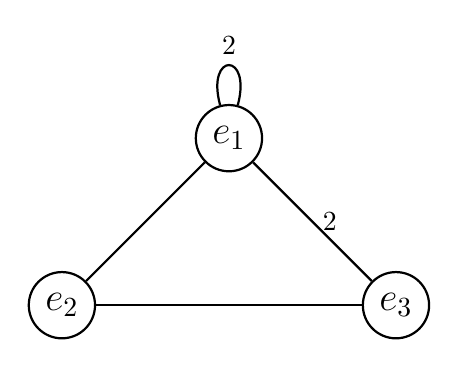
\begin{tikzpicture}[auto, node distance=3cm, every loop/.style={},
                    thick,main node/.style={circle,draw,font=\sffamily\Large\bfseries}]

  \node[main node] (1) {$e_1$};
  \node[main node] (2) [below left of=1] {$e_2$};
  \node[main node] (3) [below right of=1] {$e_3$};

  \path[every node/.style={font=\sffamily\small}];
  \path (1) edge [loop above] node {2} (1);
  \path (3) edge node [right] {} node[right] {2} (1);
  \path (1) edge (2);
  \path (2) edge (3);

\end{tikzpicture}

\caption{Graph G}

\end{center}
\end{figure}

Note - edge weights represent number of edges, default is 1.

\newpage

Question: Is G a complete bipartite graph H = (U,V,E) with the following properties:

\begin{itemize}
\item U can be a multiset
\item V can be a multiset
\item U $\cap$ V need not be empty
\end{itemize}

For the above example, the complete bipartite representation of G that we are looking for is: 
\begin{figure}[h]

\begin{center}

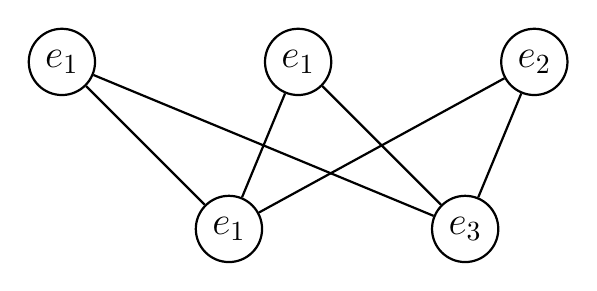
\begin{tikzpicture}[auto, node distance=3cm, every loop/.style={},
                    thick,main node/.style={circle,draw,font=\sffamily\Large\bfseries}]

  \node[main node] (1) {{$e_1$}};
  \node[main node] (2) [right of=1] {{$e_1$}};
  \node[main node] (3) [right of=2] {{$e_2$}};
  \node[main node] (4) [below right of=1] {{$e_1$}};
  \node[main node] (5) [below right of=2] {{$e_3$}};
  
  \path[every node/.style={font=\sffamily\small}];
  \path (1) edge  (4);
  \path (1) edge  (5);
  \path (2) edge  (4);
  \path (2) edge  (5);
  \path (3) edge  (4);
  \path (3) edge  (5);

\end{tikzpicture}
\caption{Graph H}

\end{center}
\end{figure}

The problem of finding whether a graph G is a complete bipartite graph under the given conditions is equivalent to finding the factors(if they exist) of a multivariate polynomial of degree 2 with no constant terms. The polynomial corresponds to the graph G whereas the factors correspond to each partition of graph H. For the above example, the multivariate polynomial is:
$(2 e_1^2 + e_1e_2 + e_2e_3 + 2 e_1e_3)$. The factors for this polynomial are $(2 e_1 + e_2)$ and $(e_1 + e_3)$.

Solving the above stated problem would give us the variables present in each operand of the long multiplication. However, we still would not know the ordering of the variables(if it exists) i.e concatenation order of the variables within the operands. We are still exploring this approach as part of our future work.


\bibliographystyle{unsrt}
\bibliography{biblio}


\end{document}

%%% Local Variables:
%%% mode: latex
%%% TeX-master: "main"
%%% End:
